\documentclass[11pt,twoside]{report}
\usepackage{preamble}
\graphicspath{{../img/ch4/}}
\setcounter{chapter}{3}


\begin{document}

\chapter{Observing Zebrafish in 3D}
\label{chapter:fish_3d}

%\epigraph{奇肱之国在其北 其人一臂三目}{\emph{山海经・海外西经}}

\section{Introduction}

This chapter presents the method to build up a system to observe a group of zebrafish in 3D, and obtain the 3D coordinates of individuals in a group of fish. The system is inspired by the pioneering work of \citeauthor{cavagna2008} \cite{cavagna2008} as well as \citeauthor{kelley2013} \cite{kelley2013}, where the 3D locations of European starlings and midges were calculated and analysed. 


The 3D observation is a difficult task. Compared to the the 2D observation introduced in chapter~\ref{chapter:fish_2d}, both the hardware and the software were more complicated for the 3D observation. Typically, we need to use multiple cameras to capture the movement of the fish, where the images were taken in a synchronised way. The calculation also needs more attention, since the optical details, such as the refraction of light at the water--air interface, will affect the final result.


Mathematically, it is important to understand the formation of the image on a camera, because we need to reverse this process to calculate the 3D locations.
For the relevant details, we refer the readers to \cite{hartley2003, ma2005}.
%The relevant details will be covered as a brief introduction of projective geometry in appendix~\ref{chapter:multi_view}. 
This chapter will instead focus on the \emph{implementation} of the ideas.
%Having finished the method section~\ref{section:method_locate_3d}, we should be confident about the calculated 3D locations.
%The accuracy and performance of my software implementation are included in this chapter.
The code responsible for the methods in this chapter is open source, and hosted on website ``GitHub'', with a project name of \href{https://github.com/yangyushi/FishPy}{yangyushi/FishPy}.


It is worth mentioning that the 3D observation method is also widely applied in the study of fluid mechanics \cite{maas1993}, dating back to the 1990s. The name of the method is formally \emph{particle tracking velocimetry}\marginfootnote{
The term ``particle tracking'' in the fluid mechanics community and the soft-matter community refers to slightly different things. The former focus on the dynamic (velocities) of the particles, while the latter focus more on the structure (coordinates) of the particles.
}
(PTV) in the fluid mechanics literatures. Therefore, the new development from the fluid mechanics community may provide opportunity to improve the animal. For instance, by applying the field-programmable gate array (\gls{FPGA}), the 2D feature selection can be performed in real time, which reduced the amount of processing time and data-storage space significantly \cite{chan2007}. 

In addition, the physicists and zoologists have pushed the boundary of technology for field observations. For instance, \citeauthor{cavagna2021} developed the system that can track the 3D movement of animals while moving the cameras with a joypad\marginfootnote{
A joypad is a controller connected to a computer, or other game consoles. In many 3D video games, the players rotate the virtual cameras in the game to explore the environment. This movement is also needed to follow animals in the field.
}, enabling researchers to follow the movement of birds for a long period of time \cite{cavagna2021}.
Another example of advanced observation techniques is the reconstruction of a group of fish in the field, with observers swimming together with the fish, while holding two cameras \cite{francisco2020me}. By incorporation the static environmental information, the movements of the cameras can be effectively estimated, which can be used to reconstruct the trajectories of the fish. 

Using the developed 3D observation system, I studied the behaviour of one adult wildtype zebrafish, as well as groups of zebrafish with different sizes ($N=2, 3, 50$). The result section presents their spatial distribution and the distribution of their pairwise distance. The observed results revealed the important interaction between the fish and the environment. The \emph{dynamic} of the system, which involves the time derivative of the locations, will be analysed and discussed in chapter~\ref{chapter:fish_analysis}.


\section{Methods}
\label{section:method_locate_3d}

This section should serve as a practical tutorial for building a multiple view 3D system to track animals. This system is capable of extracting 3D location of the fish, with three commercial cameras. Our choice is not the only technology to extract 3D information about animals. Instead, there are alternative ways to follow the movement of animals such as binding animals with global positioning system (GPS) \cite{nagy2010} and tagging the animal bodies \cite{jolles2017}. Comparing with these solutions, our method is non-invasive and relatively cheap. However, the obtained results are affected by the errors of the 2D locating of fish individuals (section \ref{section:image_process}), and the ambiguity in the stereo matching process (section \ref{section:fish_many_3d}).

\subsection{Tank Design and Hardware}
\label{section:system_3d}

\begin{SCfigure}
  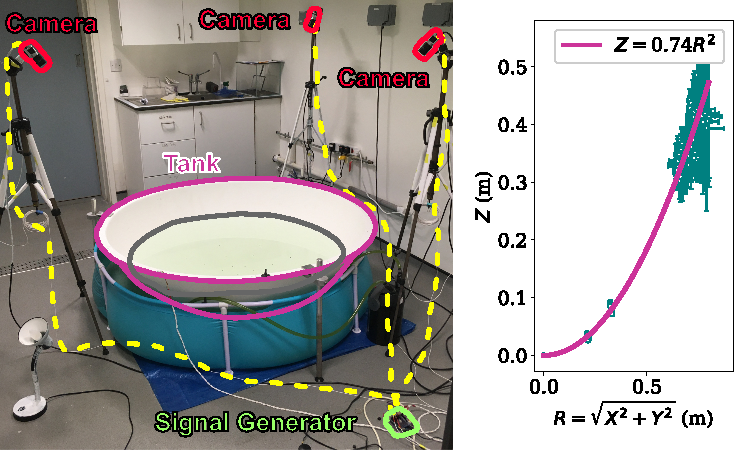
\includegraphics[width=\linewidth]{lab}
  \caption[Three dimensional fish tracking system]{
  Left: The photo of one experimental setup. Three cameras are mounted to observe the fish in the bowl-shaped tank. Time--synchronised signals were generated by an Arduino chip to trigger the cameras for capturing synchronised videos. The bowl was immersed in a bigger tank, which is a framed swimming pool. The husbandry--related equipments, such as the water filter, the heaters, the UV lamp, were placed outside the bowl but inside the bigger tank.
  Right: The measured shape of the observation tank. The scatters were markers on the tank, which were fitted by function $z=0.74 r^2$, where the unit of both $z$ and $r$ is meter.
  }
  \label{fig:lab}
\end{SCfigure}

Figure \ref{fig:lab} shows the experimental setup in the laboratory, where I mounted 3 cameras pointing to a bowl--shaped tank. This big bowl was immersed in a framed swimming pool. Synchronised signals were generated with a Arduino chip, and the cameras are able to capture time--synchronised videos with the signals. The trigger signal for the camera is a 5V pulse, being the default \texttt{HIGH} output signal of an Arduino chip.


The big, white plastic bowl was specially designed and manufactured to contain the fish. The choice of the shape was based on the fact that the fish tend to stay in the corner of the tank, when they entered an unfamiliar environment \cite{kalueff2013, mwaffo2016}. Using a bowl--shaped container prevented the aggregation at the corners. Except for the corner effect, the bowl also provides no blind zone for all of the cameras, preventing the systematic disappear and reappearing of the fish in the video.


%The zebrafish are living animals, and it is also important to provide them a suitable condition. 
In order for the zebrafish to exhibit normal behaviour, they should have water conditions comparable to those used to house them.
Typically, the fish need a temperature between 25 \degree C and 30 \degree C, and the water should be constantly filtered and sterilisation with UV light.
All of the related apparatusse were placed outside the bowl--shaped tank, but inside the swimming pool, so that they would not affect the behaviours of the fish.
The entire system was heated by two commercial heaters. The warm water was circulated into the inner bowl with a water pump. The bowl was able to exchange water with outside via small holes drilled inside. The measured temperature in the swimming pool ranges from 23 \textdegree C to 26 \textdegree C. The water circulation is turned off during observations of fish swimming.


The 3D shape of the tank was measured, so we know the exact boundary for the fish. The measurement was performed by placing markers on the surface of the tank, and then reconstruct the markers in 3D. Since the tank is rotationally symmetric around the z--axis, it is appropriate to describe its geometry in the cylindrical coordinate system with the height ($z$) and the radius ($r$). Figure~\ref{fig:lab} (Right) shows the results of the measurement, and the shape of the tank can be modelled by function $z=0.74 r^2$, where both length variables have the units of meter. The shape of the tank, together with the water level, are the boundaries for the movement of the fish.



\subsection{Locating One Fish in 3D}
\label{section:locate_3d}

\begin{SCfigure}
    \centering
    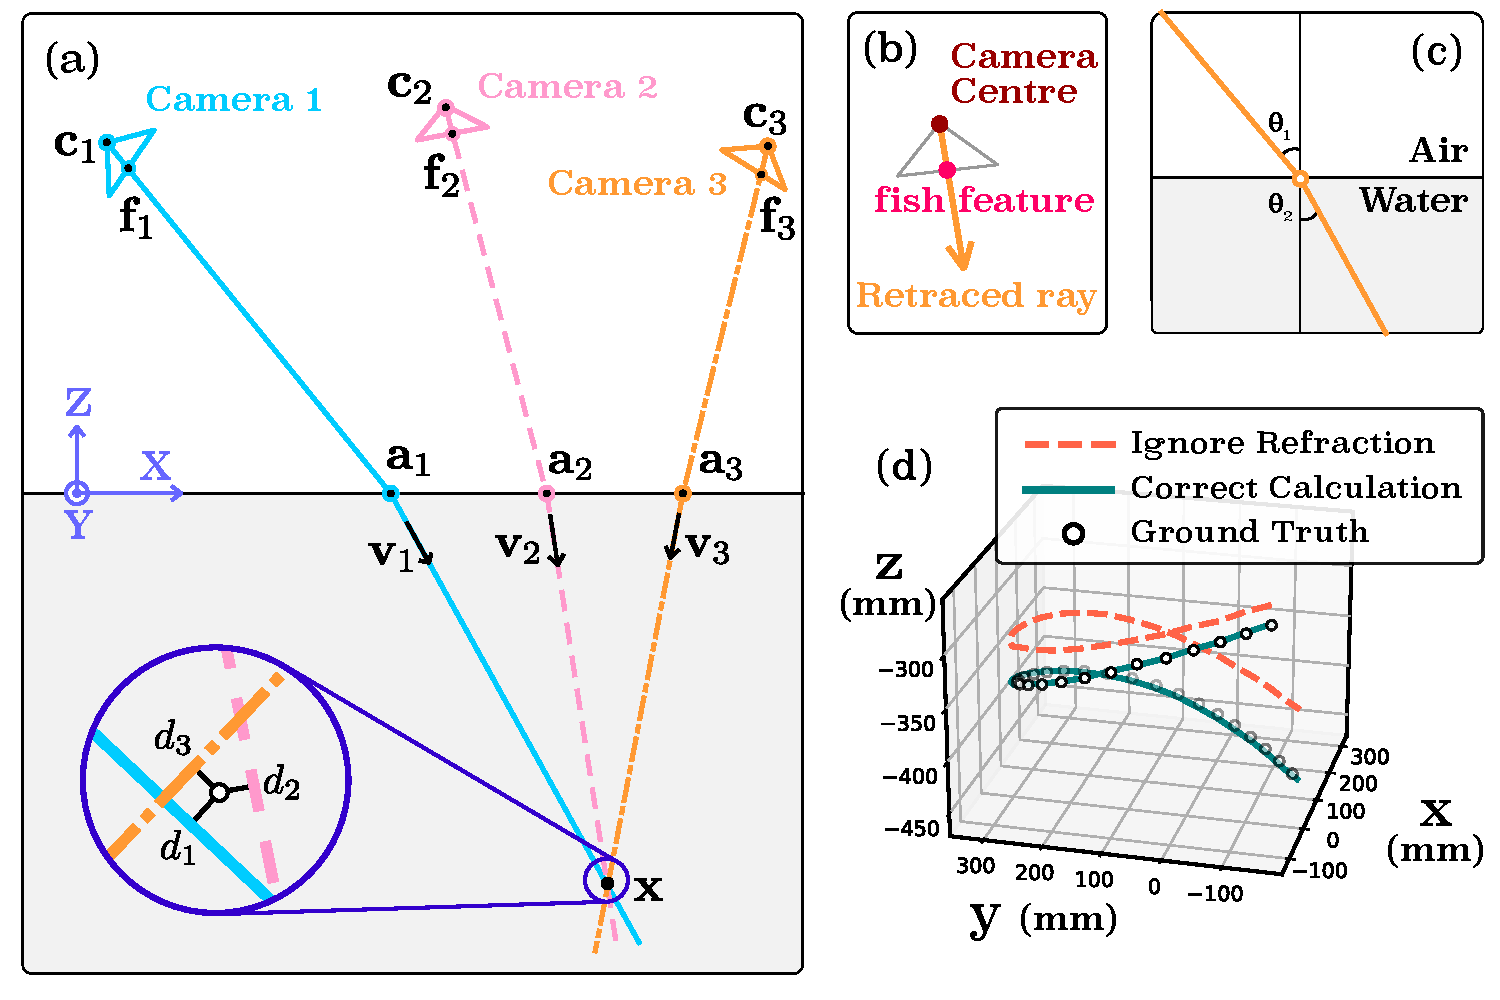
\includegraphics[width=\linewidth]{locate-one}
    \caption[The concept of tracking one fish in 3D]{\label{fig:locate-one}
        The illustrations for the concept for locating one fish in 3D.
        (a) the schematic for the calculation of the 3D fish location from three cameras. The ``intersection'' of the refracted rays were magnified, to stress the retrace distances.
        (b): The illustration of retraced ray from the 2D fish features.
        (c): The effect of the refraction;
        (d): The validation of the calculation for the 3D location of one simulated fish. The solid line is the result where the refraction is considered, and the dashed line is the calculation result that ignored the refraction effect. The scatters represent the ground truth.
    }
\end{SCfigure}



Figure~\ref{fig:locate-one} summarises the essential concept to locate the 3D position with a three camera setup. 
The task of finding the 3D positions of zebrafish consists of two parts. The first part is finding the features of fish in individual cameras, as discussed in the chapter~\ref{chapter:fish_2d}. These features corresponds to $\mathbf{f}_i \in \mathbb{R}^3$ in Fig.~\ref{fig:locate-one}(a).\marginfootnote{
The symbol $\mathbf{f}_i$ stands for the 3D location of the detected 2D features. We need the knowledge of the camera to calculate $\mathbf{f}_i$ from the features in the image. 
}
The second part is to retrace the ray from the features \gls{fi}, back to its original 3D location \gls{xi}, as illustrated in Fig.~\ref{fig:locate-one} (b).

To carry out the 3D calculation procedure, we need to know the location, orientation, and optical details about the camera. This information can be obtained with the \emph{camera calibration} \cite{zhang2000, hartley2003}.
%, which is introduced in appendix~\ref{chapter:multi_view}. 
Essentially, the knowledge of the camera can be represented by a $3 \times 4$ matrix \gls{proj_mat}, named the \emph{projection matrix}. For a 3D point $\mathbf{x} = (x, y, z)^\top$, the camera with projection matrix $\mathbf{P}_{3 \times 4}$ will project the 3D point on a 2D plane, with coordinate $(u, v)^\top$, satisfying  equation,\marginfootnote{I use column vectors consistently in this thesis. For instance, the vector $(x, y, z)^\top$ have the shape of $4 \times 1$; while the vector $(x, y, z)$ have the shape of $1 \times 4$.}

\begin{equation}
	\mathbf{P}_{3 \times 4}
	\cdot (x, y, z, 1)^\top = k (u, v, 1)^\top
\label{eq:projection}
\end{equation}

\noindent where $k$ can take any value.
%(See appendix~\ref{chapter:multi_view} for details)
With proper decomposition of $\mathbf{P}_{3 \times 4}$, it is also possible to calculate the location of the camera centre, illustrated as \gls{center} in Fig.~\ref{fig:locate-one}(a).

 Equation~\ref{eq:projection} suggests an algebraical way to calculate 3D positions from 2D features. With known \gls{proj_mat} and $(u, v)$, Eq.~\ref{eq:projection} offered 2 constrains on the values of \gls{loc3d}. Therefore, the 3D vector $\mathbf{x}$ can be uniquely determined by 2 or more ``camera + feature'' combinations.\marginfootnote{This method to find 3D location is called \emph{triangulation}.} However, the water in the fish tank will refract the light. Figure~\ref{fig:locate-one} (c) shows the effect of refraction, where the angle of incidence $\theta_1$ and the angle of refraction $\theta_2$ follows the Snell's law: $n_1 \sin\theta_1 = n_2 \sin\theta_2$. As a consequence, the calculation of $\mathbf{x}$ involves the following steps,
 
 \begin{enumerate}
 	\item For each feature $\mathbf{f}_i$, calculate its corresponding point on the water-air interface $\mathbf{a}_i$.
 	\item Calculate the direction of refracted ray $\mathbf{v}_i$.
 	\item Find the interception of multiple refracted rays, as the location of fish in 3D $\mathbf{x}$.
 \end{enumerate}


The calculation of \gls{ai} and \gls{vi} requires knowledge of the water-air interface, which was obtained during the camera calibration. Typically, we are free to choose the orientation and location of the \emph{world coordinate frame}. And I set the frame so that the water-air interface is plane $z = 0$, as plotted in Fig.~\ref{fig:locate-one}(a). This extra constrain ensures the value of $\mathbf{a}_i$ being uniquely determined by a 2D feature $(u, v)$. Following Eq.~\ref{eq:projection}:

$$
\left(
\begin{matrix}
	P_{11} & P_{12} & P_{13} & P_{14} \\
	P_{21} & P_{22} & P_{23} & P_{24} \\
	P_{31} & P_{32} & P_{33} & P_{34} \\
\end{matrix}
\right) 
\cdot
\left(
\begin{matrix}
a_x \\ a_y \\ 0 \\ 1	
\end{matrix}
\right) =
k\left(
\begin{matrix}
	u \\ v \\ 1
\end{matrix}
\right),
$$

\noindent where $\mathbf{a}_i = (a_x, a_y)^\mathrm{T}$, and $k$ is a scaling variable that can take any value. Notice there are 3 linear equations for 3 variables ($a_x, a_y$ and $k$), meaning that we can easily calculate $\mathbf{a}_i$. The incident ray can be obtained from $\mathbf{a}_i$ and corresponding \gls{cci}. Applying Snell's law, we can calculate the direction of the refracted ray, yielding $\mathbf{v}_i$. %The algorithm for this calculation is available in appendix~\ref{chapter:algorithms}.


Ideally, the knowledge of the refracted rays ($\mathbf{a}_i$ and $\mathbf{v}_i$) from different cameras yields the 3D location of the fish. Realistically, because of the errors during the 2D feature detection and camera calibration, the retraced rays will not meet each other in 3D space exactly, as pictured in the inset in Fig.~\ref{fig:locate-one}(a). Therefore, finding $\mathbf{x}$ is a minimisation problem. And the value to be minimised is the sum of distances from $\mathbf{x}$ to all the retraced rays. The distance from $\mathbf{x}$ to the retraced ray from camera $i$ is called the \emph{retraced error}, noted as \gls{reterri}. The value of $d_i$ can be calculated as


\begin{equation}
	\label{eq:retrace_err}
	d_i = \vert
	(\mathbf{x} - \mathbf{a}_i) \times \mathbf{v}_i
	\vert,
\end{equation}


\noindent where the retraced ray from camera $i$ passed through point $\mathbf{a}_i \in \mathbb{R}^3$, with the unit direction of $\mathbf{v}_i \in \mathbb{R}^3$. For the constant $\mathbf{a}_i$ and $\mathbf{v}_i$, the squared sum of the retraced error is a function of $\mathbf{x}$, written as,

$$
f(\mathbf{x}) = \sum_i{d_i^2} 
= \sum_i{\left( \vert \mathbf{x} - \mathbf{a}_i \vert^2 \; \vert \mathbf{v}_i^2 \vert - 
\vert \ (\mathbf{x} - \mathbf{a}_i) \cdot \mathbf{v}_i\ \vert^2 \right)}
$$

\noindent where the operator $\vert \cdot \vert$ represents the norm of a 3D vector. We can think of $f(\mathbf{x})$ as a scalar field (like temperature), and the minimum of the field can be found, by setting its gradient ($\nabla f$) to zero. The relation ($\nabla f = 0$) yields a set of linear equations,

\begin{equation}
	\label{eq:location_3d}
	\mathbf{M} \cdot \mathbf{x} = \mathbf{b}.	
\end{equation}

\noindent The values of $\mathbf{M} \in \mathbb{R}^{3 \times 3}$ and $\mathbf{b} \in \mathbb{R}^3$ can be calculated as,

$$
\begin{aligned}
\mathbf{M} &= \sum_i{\mathbf{T}_i} = \sum_i{
\mathbf{v}_i \cdot \mathbf{v}_i^T - 
\textrm{diag}(\mathbf{v}_i \circ \mathbf{v}_i)
} \\
\mathbf{b} &= \sum_i{
\mathbf{T}_i \cdot \mathbf{a}_i,
} \\
\end{aligned}
$$

\noindent where the symbol $\circ$ represents the Hadamard product. The function $\textrm{diag}(\mathbf{x})$ transform the vector $\mathbf{x} \in \mathbb{R}^n$ to a diagonal matrix $\mathbf{D} \in \mathbb{R}^{n \times n}$, where $D_{ii} = x_i$. Solving the equation~\ref{eq:location_3d} is easy with standard linear algebra methods such as Gaussian elimination.\marginfootnote{
Using the Python language, the solution can be found with function \texttt{numpy.linalg.solve(M, b)}. In C++ the task can be performed with \texttt{M.ldlt().solve(b)}, where both \texttt{M} and \texttt{b} are matrix and vector from the \texttt{Eigen} library.
}

Figure~\ref{fig:locate-one} (d) shows the calculation of the 3D location of simulated fish. The simulation was performed with software Blender, in which the experimental apparatus  was constructed virtually. The video was recorded with virtual cameras in the software, and the aforementioned procedure was used to calculate the fish locations. Comparing the calculation result with the known ground truth, it is clear that our calculation yields correct results. 
Since the water is relatively deep (300 - 400 mm in depth) in our experiment, the effect of the refraction could not be ignored. In Fig.~\ref{fig:locate-one} (d) we also present the consequence of ignoring the refraction, which leads to a significant deviation from the ground truth.

\begin{SCfigure}
  
\includegraphics[width=\linewidth]{locate-many}
  \caption[The concept of tracking many fish in 3D]{Tracking many fish with three cameras. The correct identity match from different views yields the intersection between the retraced rays, plotted as solid lines. The unmatched rays will not meet each other, illustrated by the dashed lines.}
  \label{fig:locate-many}
\end{SCfigure}


\subsection{Locating Many Fish in 3D}



Calculating the 3D locations of many fish requires more work than locating one fish in 3D. This is because the different fish in different views (captured by different cameras) have to be matched correctly.
An example of mismatched fish were shown in Fig.~\ref{fig:locate-many} as dashed lines.
Since the three dashed lines correspond to different fish identities, they do not meet together. It is possible to use brute-force enumeration to generate all the possible identities matches, and then discarded the invalid ones. This algorithm was summarised in algorithm~\ref{alg:locate-3d}, where all possible solutions were generated in a triple \code{for} loop. These possible solutions were validated, and the invalid values were discarded.


\begin{algorithm}
    \KwResult{A collection of valid location $\mathbf{x}$}
	\For {$i \gets 1, n_1$} {
	\For {$j \gets 1, n_2$} {
	\For {$k \gets 1, n_3$} {
	$\mathbf{x} \gets $ Solution of $\bf M \cdot x = b$\;
	
	\If {$\mathbf{x}$ is valid}
		{put $\mathbf{x}$ in Result}
	}}}

\caption{Brute force algorithm for locate many fish in 3D.}
\label{alg:locate-3d}
\end{algorithm}


Naively, we will use the retraced error (Eq.~\ref{eq:retrace_err}) to validate every solution $\mathbf{x}$. The operation is summarised in algorithm~\ref{alg:validate-naive}, where a threshold value of $d_m$ is used to discard the solutions with large retraced errors.

\begin{algorithm}

$d_i \gets (\mathbf{x} - \mathbf{a}_i) \times \mathbf{v}_i$\;
$d_j \gets (\mathbf{x} - \mathbf{a}_j) \times \mathbf{v}_j$\;
$d_k \gets (\mathbf{x} - \mathbf{a}_k) \times \mathbf{v}_k$\;
\If {$(d_i + d_j + d_k)/3 < d_m$}
	{\textbf{return} True}
\Else {\textbf{return} False}

\caption{Validate a 3D location with retraced error.}
\label{alg:validate-naive}
\end{algorithm}

However, this method is inadequate because of the correlation of the retraced error and the location of the fish: The retraced error is larger when the fish is deeper in the water. Such correlation is exhibited in Fig.~\ref{fig:compare-error}, with simulated data. The correlation between error values and depth will lead to a systematic error, where the fish closer to the water-air interface will be preferred. Such correlation might originate from the arrangement of the camera. As they were pointed to the water from above, the retraced rays will be closer to each other when they were close to the water-air interface (see Fig.~\ref{fig:locate-many}).

\marginpar{
\centering
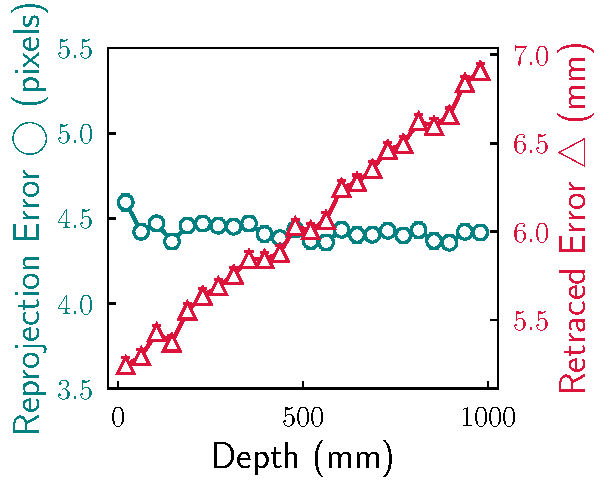
\includegraphics[width=\marginparwidth]{compare-error}
\captionof{figure}[]{
  	The reprojection error ($\epsilon$) and retraced error ($d_i$ in Eq.~\ref{eq:retrace_err}) as a function of fish location.
	}
\label{fig:compare-error}
}

To overcome such bias, we can use the \emph{reprojection error} \cite{hartley2003} to separate the valid and invalid solutions of Eq.~\ref{eq:location_3d}. The reprojection error is defined as

\begin{equation}
	\epsilon_i	= \left\vert 
	( u_\mathbf{x}, v_\mathbf{x} )^\top
	- (u, v)^\top \right\vert
\label{eq:reproj-err}
\end{equation}

\noindent where $(u, v)^\top$ represents the 2D fish features in the camera, and $(u_\mathbf{x}, v_\mathbf{x})^\top$ represents the projection of solution $\mathbf{x}$ to camera $i$. The essential calculation for \gls{reperr} is to re-project a 3D point $\mathbf{x}$ back to the camera correctly, with the optical details being considered explicitly.
%(The calculation for the reprojection is introduced in appendix~\ref{chapter:algorithms}.)
The reprojection error exhibits no correlation with respect to the location of the fish, as shown in Fig.~\ref{fig:compare-error}, which makes it a suitable choice for the validation of fish locations $\mathbf{x}$.\marginfootnote{
Unfortunately, the reprojection error can not be used to find $\mathbf{x}$. The minimisation of $\sum_i\epsilon_i^2$ will not yield a set of linear equations like Eq.~\ref{eq:retrace_err}.
} The algorithm for the validation with the reprojection error is summarised in algorithm~\ref{alg:validate}.


\begin{algorithm}

$\epsilon_i \gets$ reprojection-error($\mathbf{x}$, i)\;
$\epsilon_j \gets$ reprojection-error($\mathbf{x}$, j)\;
$\epsilon_k \gets$ reprojection-error($\mathbf{x}$, k)\;

\If {$(\epsilon_i + \epsilon_j + \epsilon_k)/3 < d_m$}
	{\textbf{return} True}
\Else {\textbf{return} False}

\caption{Validate 3D location with reprojection error.}
\label{alg:validate}
\end{algorithm}



The result of 3D locating of 10 simulated fish were shown in Fig.~\ref{fig:locate-many-valid}. The simulated 3D data were reprojected to different cameras. These projected coordinates were mixed with Gaussian noise, forming the 2D features, to mimic the real life feature measurement. The information of the identity across different cameras was removed. Then our 3D locating method (algorithm~\ref{alg:locate-3d} and \ref{alg:validate}) was used to calculate the 3D locations from these 2D features. It is clear from Fig.~\ref{fig:locate-many-valid} that all of the 10 fish were correctly located, even in the existence of 2D measurement errors.


\begin{SCfigure}
  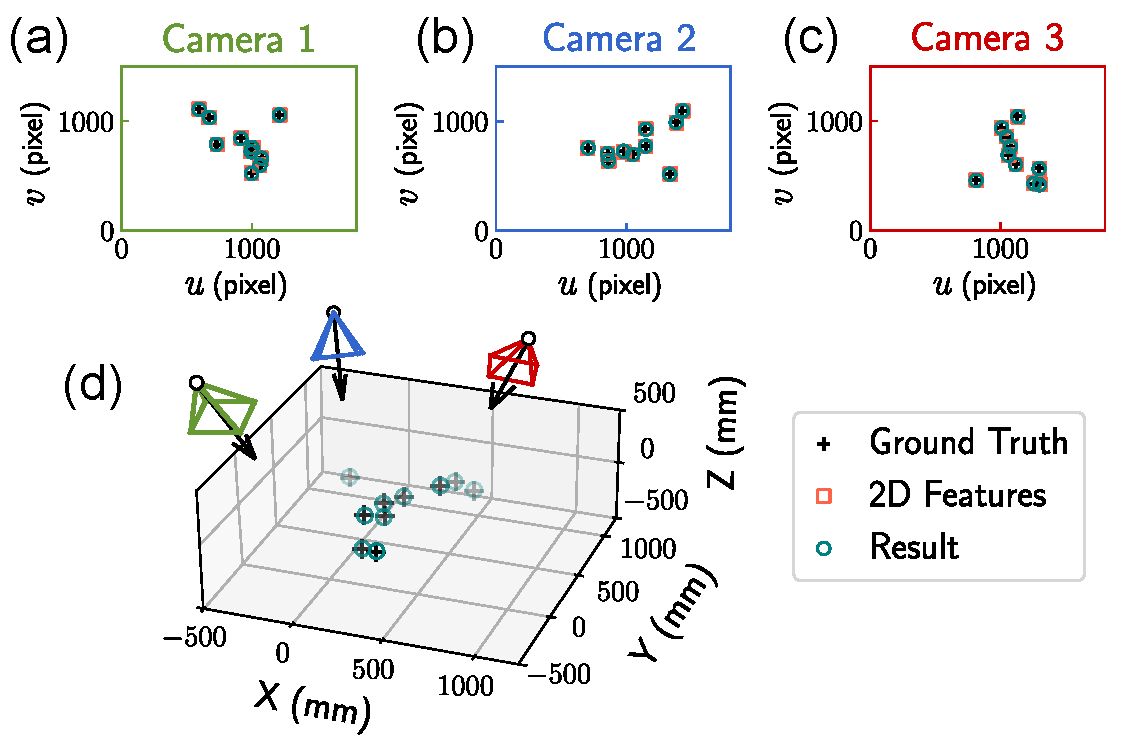
\includegraphics[width=\linewidth]{locate-many-valid}
  \caption[Three dimensional tracking result of simulated data]{
    Calculating the 3D locations of 10 simulated fish locations.
  	(a)-(c): the location captured by different cameras. The cross markers represent the known ground truth. The squares represent the measured 2D features, containing Gaussian noise. The circles represent the projection of the calculated 3D fish locations.
  	(d): the ground truth and the calculated fish location in 3D.
  }
  \label{fig:locate-many-valid}
\end{SCfigure}


\subsection{Optimising the Stereo Matching}
\label{section:stereo-opt}

It is worth mentioning an optimisation idea proposed by \citeauthor{attanasi2015b} to refine the stereo matching of fish identities\marginfootnote{
The same process is called stereoscopic linking in \cite{attanasi2015b}.
}
across different cameras \cite{attanasi2015b}. The idea is to minimise the sum of reprojection error while ensuring the existence of all fish features in the valid solutions. 
For instance, in a collection of valid 3d locations \gls{xijk}, we want to minimise the sum of their corresponding reprojection errors (Eq.~\ref{eq:reproj-err}), by discarding some ``bad'' solutions. The result of this process is a subset of \gls{xijk}, noted as \gls{xijkopt}.
And the solutions in \gls{xijkopt} are termed as the \emph{optimised solutions}.

Without any constraint, the result of minimised error will be an empty set, meaning $\{ \mathbf{x}_{ijk} \}_\textrm{opt} = \emptyset$. This is not very effective because the algorithm will trivially return nothing. A sensible way to remedy this situation is to enforce some kind of constraint, to ensure the existence of good results. The essence of the idea from \citeauthor{attanasi2015b}, is the following constraint,

$$
\forall i \; \sum_{j k} x_{i j k} \geq 1,
\forall j \; \sum_{k i} x_{i j k} \geq 1,\;\textrm{and}\;
\forall k \; \sum_{i j} x_{i j k} \geq 1,
$$

\noindent where $i, j, k$ are the indices for features in the 3 cameras. The symbol $x_{ijk}$ represents a 3D boolean tensor, whose elements can take values of $0$ or $1$. If the value of $x_{ijk} = 1$, then the feature $i$ in camera 1, the feature $j$ in camera 2, and the feature $k$ in camera 3 will form a optimised solution (in $\{ \mathbf{x}_{ijk} \}_\textrm{opt}$). Formally, the task can be written as a \emph{linear programming} problem, written as,

\begin{equation}
\begin{aligned}
	\textrm{Minimize} 
	&& \sum_{ijk}{\epsilon_{ijk}} \\
	\textrm{Subject to}
	&& \forall i \; \sum_{j k} x_{i j k} \geq 1, \\
	&& \forall j \; \sum_{k i} x_{i j k} \geq 1 \\
	&& \forall k \; \sum_{i j} x_{i j k} \geq 1
\end{aligned}
\label{eq:stereo-opt}
\end{equation}

\noindent This problem can be solved effectively by modern optimisation libraries, and they give satisfying results without significant increase in the computation time.


\begin{tcolorbox}[
title=What is ``Linear Programming'',
enlarge bottom by=0.5em,
enlarge top by=0.5em,
parbox=false
]
The method \emph{linear programming} is a very useful optimisation method. We can use it to find the maximum value of a function, plus a set of linear constraints. Equation~\ref{eq:stereo-opt} is an example of the problem that linear programming could solve. To actually solve the problem, we need to apply some complicated algorithms like the \emph{simplex algorithm}. The details of these algorithms are beyond the scope of this thesis.

Practically, we can use many existing libraries and softwares to solve the linear programming problems. I used the CPLEX package from the company IBM to carry out the linear programming calculation, following \cite{attanasi2015b}. The package is not open-source, but offers free academic licence for researchers. Being a powerful solver, the CPLEX package can solve optimisation problems with quadratic constraints. We will utilise this feature in chapter~\ref{chapter:fish_analysis} to remove overlapping particles.

Confusingly, the ``programming'' in the name does not refer to computer programmes. It originates from its first application, where George B. Dantzig was invited to solve an assignment problem for American military after world war II \cite{dantzig2002}. Internally, the schedules in the army was called the programme. \citeauthor{dantzig2002} formulated the problem into a system of linear inequalities, and published a paper under the name of \emph{Programming in a Linear Structure}. Later, he took the suggestion from a friend, and changed the name of this method to \emph{linear programming}, while strolling on the Santa Monica beach in the summer of 1948 \cite{dantzig2002}.
\end{tcolorbox}


\subsection{Assessing the Algorithm}

For the experimental videos, the realistic accuracy of the algorithm depends on the distribution of the 2D error as well as the error in the camera calibration process.
It is difficult to estimate the effects of theses uncertainties theoretically, and we refer the readers to \cite{theriault2014} for relevant studies.

Practically, we can inspect the reprojected locations $(u_\mathbf{x}, v_\mathbf{x})$ to check the accuracy.
An example is shown Fig.~\ref{fig:locate-performance} (a), where the reprojected 3D tracking result as well as the detected 2D features were plotted on top of the captured image from one camera.
The distribution of the reprojection error $\epsilon$ was plotted in Fig.~\ref{fig:locate-performance} (c), featuring a peak at $\sim$ 2 pixels.
The distribution of $\epsilon$ indicates that the reprojected coordinates $(u_\mathbf{x}, u_\mathbf{x})$ are close to the 2D features $(u, v)$.
Such proximity should give us confidence about the algorithm on the experimental data. Notably, the 3D locating algorithm is even capable of discarding some invalid 2D features, since their corresponding invalid 3D result would be discarded by algorithm~\ref{alg:validate}.


\begin{SCfigure}
  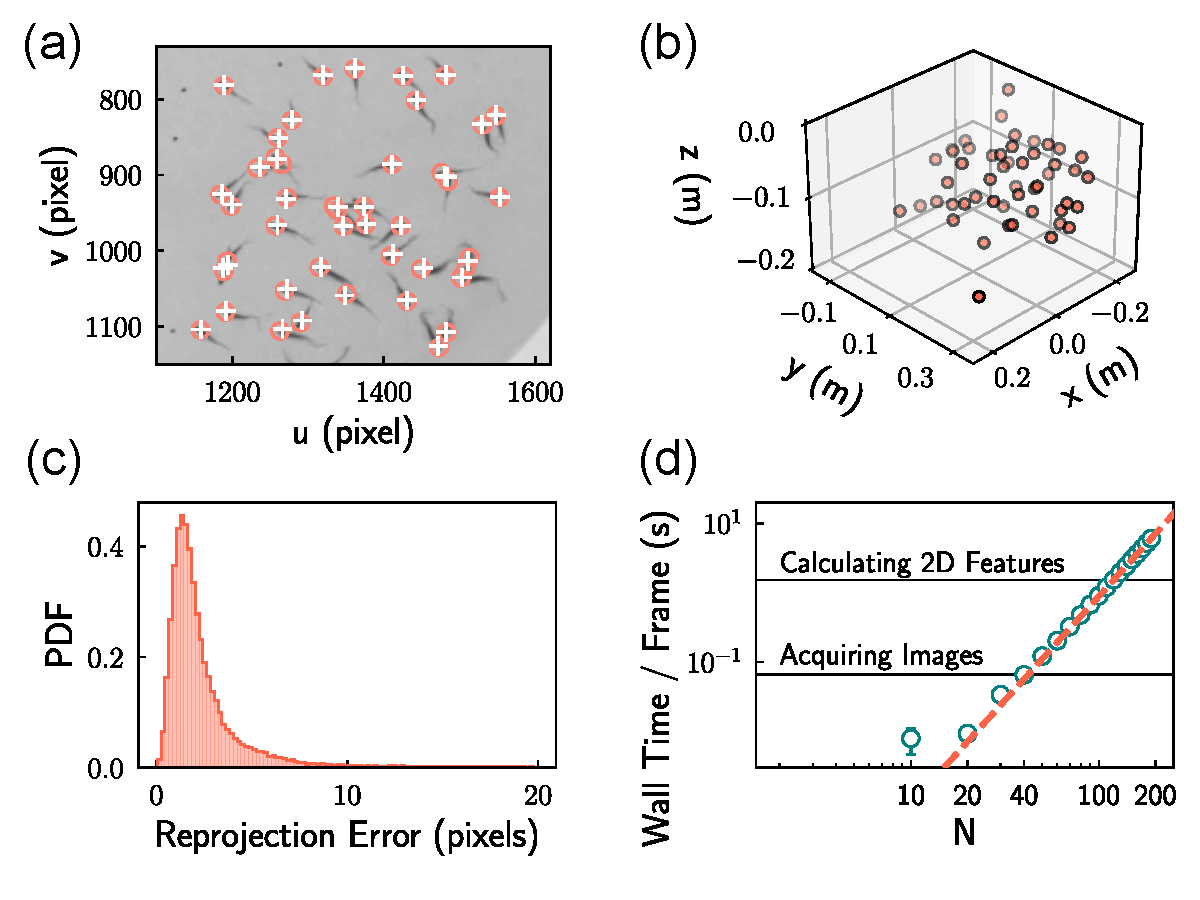
\includegraphics[width=\linewidth]{locate-perform}
  \caption[Performance of the 3D locating method]{
  (a) An image of 40 zebrafish in the experimental setup.  The detected 2D features, corresponding to $(u, v)$ in Eq.~\ref{eq:reproj-err}, were plotted as white circles. The reprojected 3D tracking result, correspond to $(u_\mathbf{x}, v_\mathbf{x})$ in Eq.~\ref{eq:reproj-err}, were plotted as the red cross markers. We cropped the image to focus on the fish group. 
  (b) The reconstructed 3D locations of 40 zebrafish from three different cameras.
  (c) The distribution of reprojection error $\epsilon$.
  (d) The wall time of the 3D locating algorithm for different numbers of fish. The dashed line shows the cubic fitting ($y = a x^3 + b$).
  }
\label{fig:locate-performance}
\end{SCfigure}


The complexity of the 3D locating algorithm is $\mathcal{O}(n^3)$, because of the triple \code{for} loop in algorithm~\ref{alg:locate-3d}. The performance of the algorithm is shown in Fig~\ref{fig:locate-performance} (d), where the wall time\marginfootnote{
The wall time refers to time spent in real life, counted by a clock on the ``wall''
} exhibits the expected cubic increase.
 To get even better performance, one needs to improve the algorithm to reduce the complexity from $\mathcal{O}(n^3)$. A possible option is to exploit the epipolar geometry \cite{hartley2003}, which can reduce the complexity of the algorithm. Further optimisation of the 3D locating algorithm will be an important task of this project in the future.


Even though the 3D locating algorithm was not optimised, it is good enough\marginfootnote{
To achieve high performance, a fast programming language is important: the result in Fig.~\ref{fig:locate-performance} was from an implementation using the C++ language, which is 1,000 times faster than a Python implementation.
} for relatively small group sizes (less than 100 fish).
For these small numbers, the bottleneck of the calculation is the 2D feature detection, which took about 2s for each frame.
With an image acquisition frequency of 15 FPS, the 3D locating calculation for group size $<$ 40 can even be performed in real time, if the 2D feature calculation time can be decreased dramatically.



\section{Results}
\label{section:observe-3d-result}

The 3D tracking yields the positions of the fish. From the positions, we can estimate the spatial distribution, and measure the structure of a group of fish.


\subsection{A Single Fish}
\label{section:fish_1_3d}


Figure~\ref{fig:density_3d_fish_1} (a) shows the joint probability density function (\gls{PDF}) of the $x$ and $z$ coordinates of the fish, noted as \gls{pdfxy}. This spatial distribution shows that the fish tend to stay in the bottom of the tank. We observe this behaviour repeatedly, when the fish were subjected to a new environment. It is likely to be related to the ``depth preference'' of zebrafish \cite{kalueff2013}, where the fish prefer deep water naturally. In addition, the increasing anxiety would also drive the fish to go to the bottom of the tank \cite{cachat2011, cachat2019}.


The distribution of the planer radius, $r=\sqrt{x^2 + y^2}$ is shown in Fig.~\ref{fig:density_3d_fish_1} (b), noted as $f_R(r)$. The shape of \gls{pdfr} is affected by the geometry of the tank. To understand the effect of this boundary, we calculated the distribution of the ideal gas particles, distributed uniformly inside the fish tank (see chapter~\ref{chapter:fish_model} for details). Compared to the ideal gas particles, the distribution of $r$ is closer the the centre. The shifted distribution of the fish is related to their depth preference, since the fish will be forced to the central region of the tank as they swim deeper in the water.
There are two peaks in $f_R(r)$, and this bimodal feature can be explained by the holes drilled on the tank, which will be discussed in section~\ref{section:holes}.

The distribution of $z$ component of the coordinate of the fish, noted as \gls{pdfz}, is shown in Fig.~\ref{fig:density_3d_fish_1} (c), which presents a very sharp peak around $z = 0$ m.
To get a better understanding of the fish, we calculated the \emph{excess probability density function}, \gls{pdfexz}, as

\begin{equation}
	f_Z^\mathrm{ex}(z) = \frac{f_Z^\mathrm{fish}(z)}{f_Z^\mathrm{id}(z)}
\label{eq:dist_excess}
\end{equation}

\noindent where the term $f_Z^\mathrm{fish}(z)$ represents the height distribution of the fish, while $f_Z^\mathrm{id}(z)$ represents the distribution of the ideal gas particles. The logarithm of $f_Z^\mathrm{ex}(z)$ is shown in Fig.~\ref{fig:density_3d_fish_1} (d), featuring a linear decay of the peak, and a subsequent tail.
This initial exponential decay is surprising, and it is reminiscent of the height distribution of one colloidal particle, under the gravitational field \cite{biben1993, royall2007prl}.  
We can fit this exponential decay with the following function,

\begin{equation*}
f_Z^\mathrm{ex}(z) = a \exp\left( \frac{z}{\xi_g} \right)
\end{equation*}

\noindent where $a$ is free parameter, and \gls{xig} is a length scale related to the depth preference of the fish. The value of $\xi_g$ is a measure of the ``effective gravity'' exhibited by fish, that is related to its depth preference. For one adult zebrafish, the value of $\xi_g$ is 1.2 cm. The effective gravity for the fish will be further discussed in chapter~\ref{chapter:fish_model}.


\begin{SCfigure}
  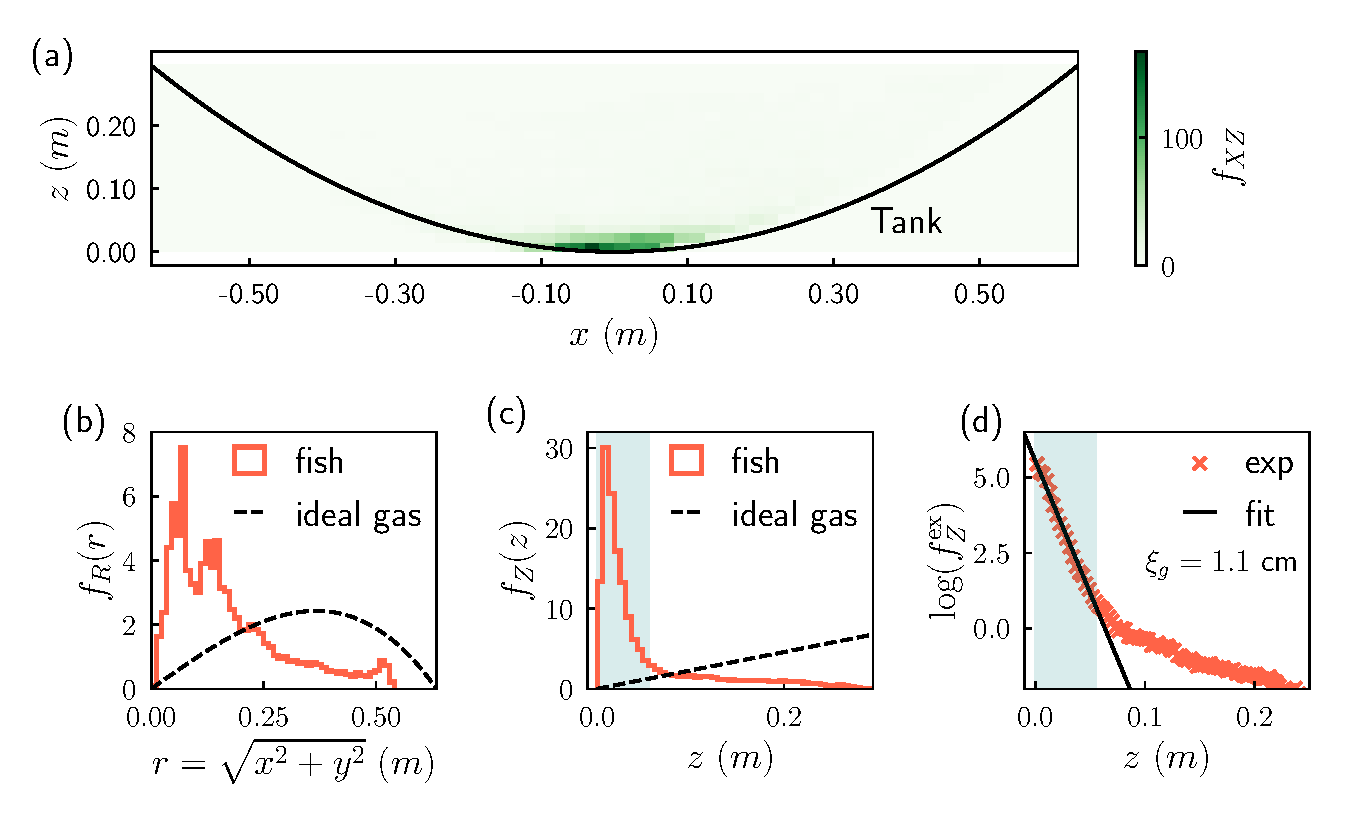
\includegraphics[width=\linewidth]{density-one-fish}
  \caption[The 3D spatial distribution of one fish]{
  The spatial distribution of one zebrafish.
  (a) The joint probability density function of $x$ and $z$ components of the fish.
  (b) The PDF for the planer radius $r$ of the fish. The dashed line shows the same PDF for the ideal gas particles distributed uniformly in the tank.
  (c) The PDF for the $z$ component of the fish. The dashed line shows the same PDF for the ideal gas particles distributed uniformly in the tank.
  (d) The semi-log plot of the excess PDF, $f_Z^\mathrm{ex}$ in Eq.~\ref{eq:dist_excess}, for the $z$ component for the fish. Fitting its initial decay revealed a lengthscale of 1.1 cm. The region of the initial decay is heighlighted in (c) and (d).
}
  \label{fig:density_3d_fish_1}
\end{SCfigure}


\subsection{Two Fish}
\label{section:fish_2_3d}


The spatial distribution of 2 zebrafish is presented in Fig~\ref{fig:density_3d_fish_2}. The behaviour of two fish is similar to that of one fish, exhibiting the typical depth preference. However, the distribution of two fish is broader compared to that of one fish.
The broader distribution indicates an increased randomness, which might related to the a decreased level of anxiety\marginfootnote{
To the best of my knowledge, there is no direct proof to suggest that zebrafish perceive less danger in a larger group. It is a reasonable speculation, since zebrafish form  groups naturally in the wild \cite{shelton2020}.
}, as the fish were swimming in pairs. In other words, one fish might be very vigilant in a new environment, exhibiting the anxiety-driven depth preference \cite{cachat2011}, which leads to a narrow distribution of $f_Z(z)$. For a pair of fish, this depth preference was reduced. The fitting result of $f_Z^\mathrm{ex}(z)$ yields a $\xi_g$ value of 1.8 cm, which is larger than the $\xi_g$ value of one fish (1.2 cm), as a result of reduced depth preference.

\begin{SCfigure}
  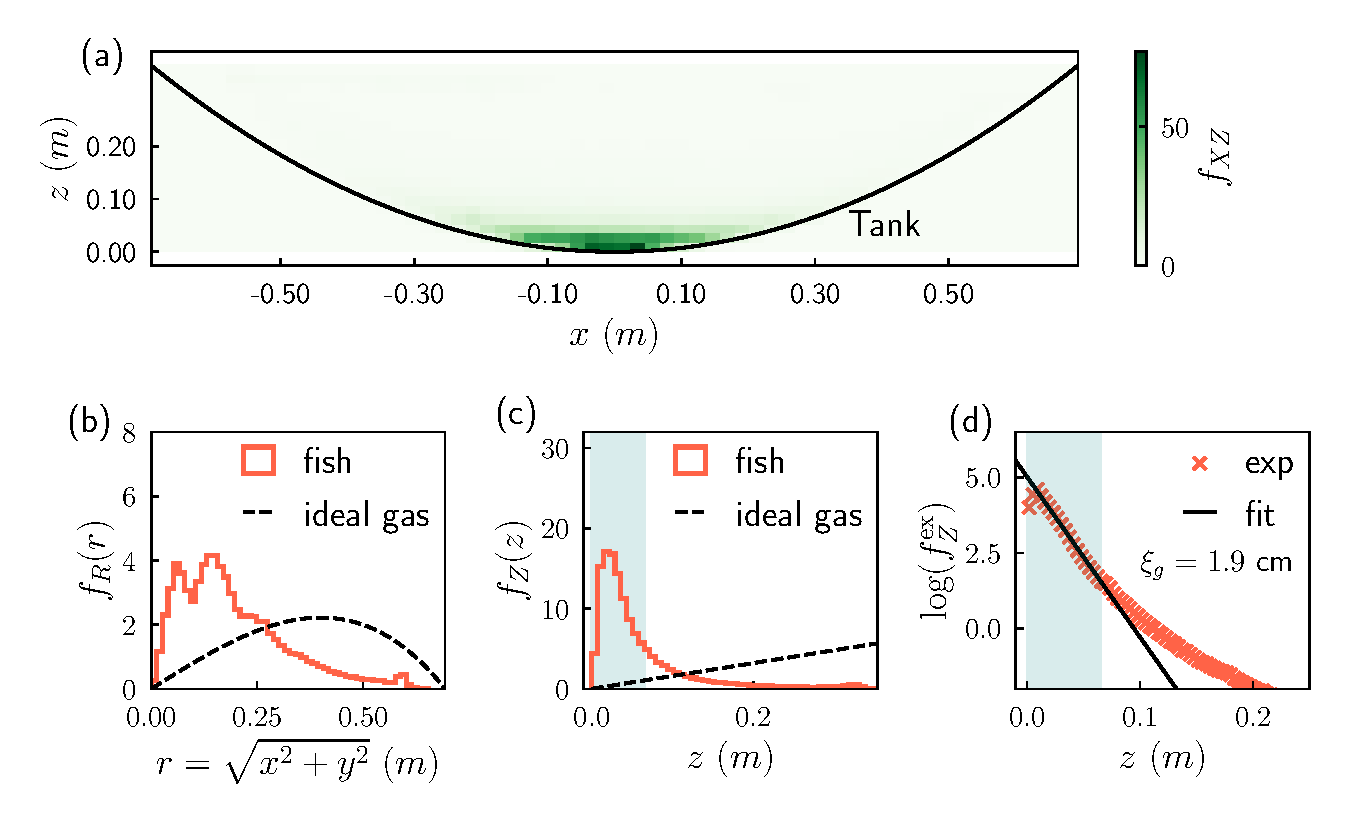
\includegraphics[width=\linewidth]{density-two-fish}
  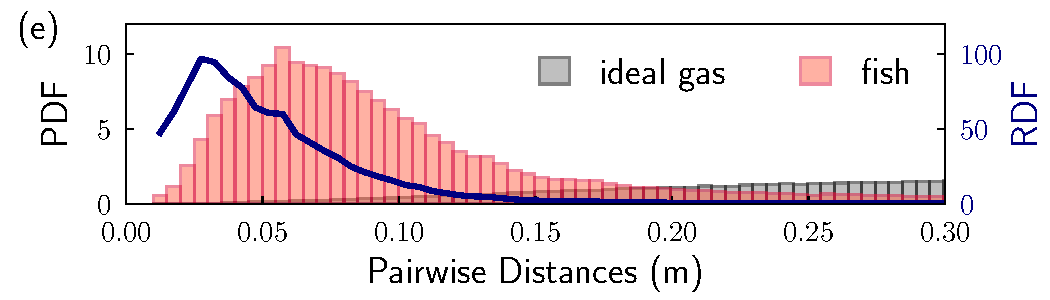
\includegraphics[width=0.9\linewidth, outer]{pdist-2fish}
  \caption[The 3D spatial distribution of two fish]{
  The spatial distribution of two adult zebrafish.
  (a) The joint probability density function of $x$ and $z$ components of the fish.
  (b) The PDF for the planer radius $r$ of the fish. The dashed line shows the same PDF for the ideal gas particles distributed uniformly in the tank.
  (c) The PDF for the $z$ component of the fish. The dashed line shows the same PDF for the ideal gas particles distributed uniformly in the tank.
  (d) The semi-log plot of the excess PDF, $f_Z^\mathrm{ex}$ in Eq.~\ref{eq:dist_excess}, for the $z$ component for the fish. Fitting its initial decay revealed a lengthscale of 1.9 cm. The region of the initial decay is heighlighted in (c) and (d).
  (e) The PDF of pairwise distances of the fish and the ideal gas particles in the tank. The ratio of the two, the radial distribution function (RDF), is plotted as a solid line.
  }
  \label{fig:density_3d_fish_2}
\end{SCfigure}

The fish-fish interaction can be probed by the distribution of the pairwise distances as well as the radial distribution function (RDF), as discussed in chapter~\ref{chapter:fish_2d}. The probability density function (PDF) of the pairwise distance of 2 fish was shown in Fig.~\ref{fig:density_3d_fish_2}, along with the corresponding PDF of the ideal gas particles uniformly distributed in the fish tank. The PDFs of the fish distance exhibit a peak around 5 cm, which is dominated by the inhomogeneity of the density distribution.

The RDF of 2 fish in the system exhibits a peak around 0.03m, with a hight value of $\sim$ 100. The hight value is significantly larger, comparing with the RDF peak height of 2 fish in 2D.
This is likely due to the depth preference of the fish that generated more significant density inhomogeneity. In other words, the fish appear to swim together in the bottom part of the tank. But the behaviour was not driven by the (biological) fish-fish attraction. Instead, these fish were just bounded together by their interaction with the environment, i.e. the depth preference. This bias induced by the depth preference can be corrected with advanced sampling method, which will be covered in chapter~\ref{chapter:fish_analysis}.


\subsection{Three Fish}
\label{section:fish_3_3d}

The spatial distribution of 3 zebrafish is presented in Fig~\ref{fig:density_3d_fish_3}. Being similar to the 1-fish and 2-fish system, a group of 3 zebrafish presents the depth preference, indicated by the biased joint PDF of $z$ and $z$ components of the fish coordinates. The PDFs ($f_Z(z)$, $f_R(r)$, and $f_{XZ}$) of 3 fish is very similar to the results from 2 fish experiments. This similarity was also observed in the 2D experiments (section~\ref{section:fish_2_2d}).

The distribution of the pairwise distance of 3 zebrafish exhibits one peak around 0.08m. The length scale matched the size of the high-density blob in Fig.~\ref{fig:density_3d_fish_3} (a), thanks to the depth preference of the fish. The RDF of 3 fish is similar to the RDF of 2 fish, with a peak at around 0.03 m. The height of the peak is close to 100, due to the depth preference of the fish, as discussed in section~\ref{section:fish_2_3d}.

\begin{SCfigure}
  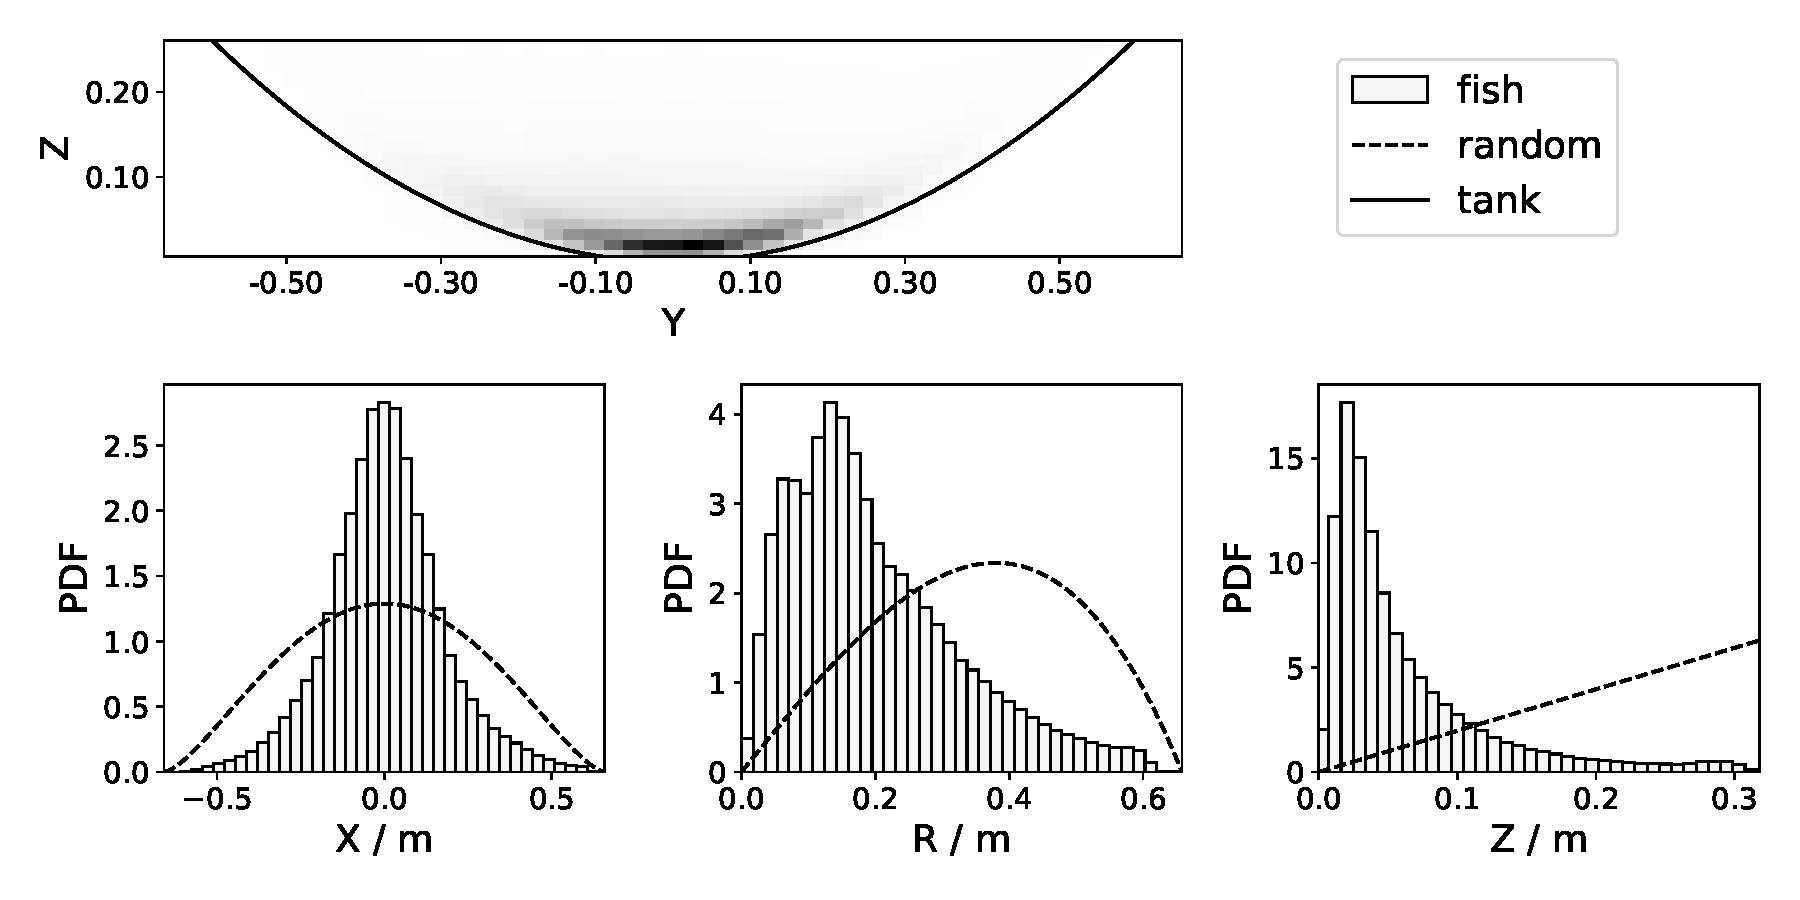
\includegraphics[width=\linewidth]{density-three-fish}
  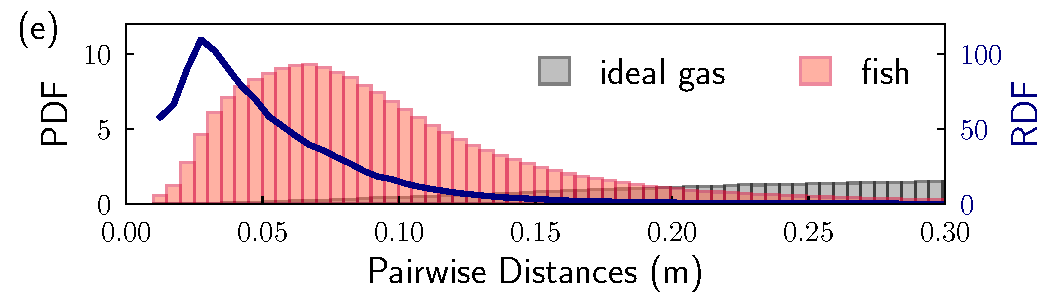
\includegraphics[width=0.9\linewidth, outer]{pdist-3fish}
  \caption[The 3D spatial distribution of three fish]{
  The spatial distribution of three adult zebrafish. 
  (a) The joint probability density function of $x$ and $z$ components of the fish.
  (b) The PDF for the planer radius $r$ of the fish. The dashed line shows the same PDF for the ideal gas particles distributed uniformly in the tank.
  (c) The PDF for the $z$ component of the fish. The dashed line shows the same PDF for the ideal gas particles distributed uniformly in the tank.
  (d) The semi-log plot of the excess PDF, $f_Z^\mathrm{ex}$ in Eq.~\ref{eq:dist_excess}, for the $z$ component for the fish. Fitting its initial decay revealed a lengthscale of 1.8 cm. The region of the initial decay is highlighted in (c) and (d).
  (e) The PDF of pairwise distances of the fish and the ideal gas particles in the tank. The ratio of the two, the radial distribution function (RDF), is plotted as a solid line.
  }
  \label{fig:density_3d_fish_3}
\end{SCfigure}


\subsection{Many Fish}
\label{section:fish_many_3d}

Figure~\ref{fig:density_3d_fish_50} shows the spatial distribution of 50 adult zebrafish, as well as the distribution of their pairwise distances and the RDF. The depth preference is obvious for a group of 50 fish, as shown in the joint PDF of $x$ and $z$ components of the fish coordinates.
However, the distribution is more homogeneous comparing with the 1/2/3 fish results. This homogeneity could be the result of reduced depth preference, as the $\xi_g$ value for 50 zebrafish is larger than that of the 1/2/3 fish. Biologically, the reduction of depth preference (the increase of $\xi_g$) can be explained by our assumption, that the fish perceive less danger in a larger group.

The distribution of the $z$ component, interestingly, exhibits two separated peaks. One of the peak is close to $z = 0\ m$ which can be explained with the depth preference. The other peak is located at $z = 0.35\ m$, which corresponds to the top of the tank. This suggests the fish were also attracted by the water-air interface. Such bimodal distribution is likely due to the biological preference of the fish, which will be further analysed in chapter~\ref{chapter:fish_analysis}.

The 50 zebrafish also shows a broad distribution for their pairwise distances. This can be explained by the reduced density inhomogeneity of the fish. Consequently, the group of 50 fish appears to be less cohesive, indicated by the absence of sharp peak in their RDF, as shown in the bottom panel of Fig.~\ref{fig:density_3d_fish_50}. The observation that a large group of fish exhibits less cohesion and less spatial inhomogeneity, was also captured by the 2D fish experiments shown in section~\ref{section:fish_50_2d}.


\begin{SCfigure}
  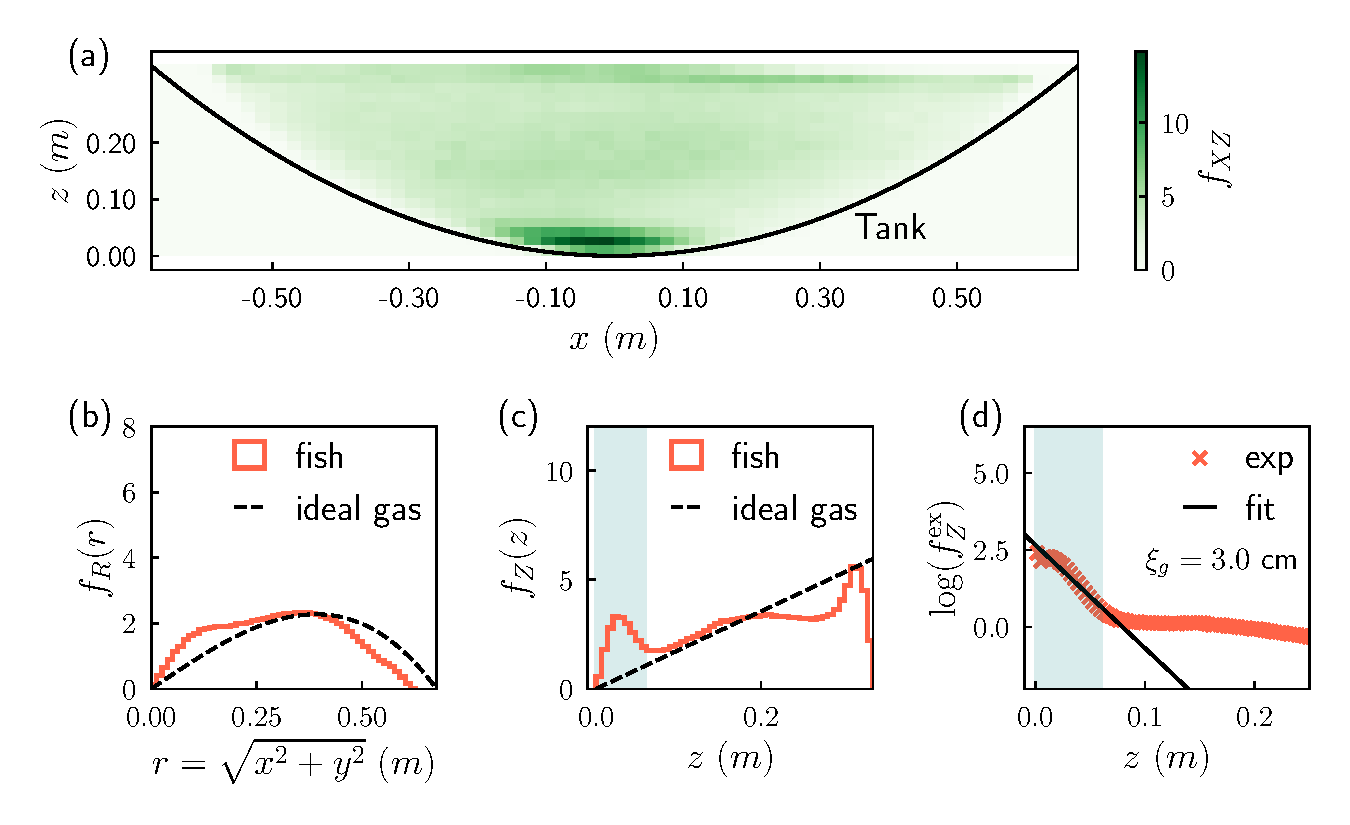
\includegraphics[width=\linewidth]{density-fifty-fish}
  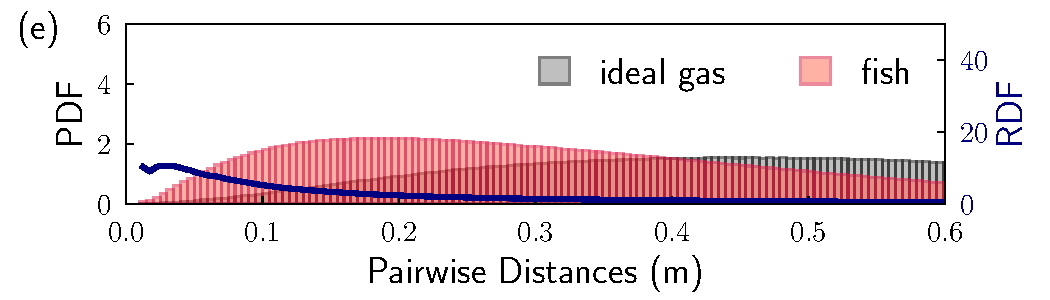
\includegraphics[width=0.9\linewidth, outer]{pdist-50fish}
  \caption[The 3D spatial distribution of 50 zebrafish]{
  The spatial distribution of fifty adult zebrafish. 
  (a) The joint probability density function of $x$ and $z$ components of the fish.
  (b) The PDF for the planer radius $r$ of the fish. The dashed line shows the same PDF for the ideal gas particles distributed uniformly in the tank.
  (c) The PDF for the $z$ component of the fish. The dashed line shows the same PDF for the ideal gas particles distributed uniformly in the tank.
  (d) The semi-log plot of the excess PDF, $f_Z^\mathrm{ex}$ in Eq.~\ref{eq:dist_excess}, for the $z$ component for the fish. Fitting its initial decay revealed a lengthscale of 3.0 cm. The region of the initial decay is highlighted in (c) and (d).
  (e) The PDF of pairwise distances of the fish and the ideal gas particles in the tank. The ratio of the two, the radial distribution function (RDF), is plotted as a solid line.

  }
  \label{fig:density_3d_fish_50}
\end{SCfigure}


\subsection{The Holes on the Tank}
\label{section:holes}

\marginpar{
\centering
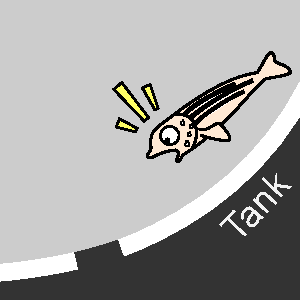
\includegraphics[width=\marginparwidth]{hole}
The holes on the tank affected the zebrafish.
}

The holes drilled on the surface of the tank had an unexpectedly large effect on the spatial distribution of the zebrafish. These holes were designed for the circulation of the water in the tank. They appear as black dots in Fig.~\ref{fig:density-holes} (right). However, the location of these holes matched the $R$ values of the density distribution, where the discontinuous singularity happens, as shown in Fig~\ref{fig:density-holes} (left). This indicates that the fish actively avoids swimming on top of these holes.

For the distribution of 1 fish, the fish-hole interaction is very significant, indicated by a very clear separation of peaks around $R=0.1$. Such separation is less significant in from the result of 2 fish and 3 fish experiments. For 50 fish, the effect of the holes is not observed in Fig.~\ref{fig:density-holes}. The result is consistent with the observation in 2D, were the fish-tank interaction dominates the 1/2/3 fish behaviour, while the fish-fish interaction dominates the behaviour of 50 fish. Such observation indicates the necessity for the large group animal behaviour experiments, if we are interested in the interaction between animal individuals.

This information about the fish-tank interaction is important for the purpose of the modelling. In chapter~\ref{chapter:fish_model} we will show that a small group of fish can be modelled as a system in equilibrium with pairwise interaction, under the influence of the tank, the gravity, as well as the holes. The Boltzmann energy weight, as a result of our equilibrium assumption for the system, gives a good match for the observed spatial distribution.


\begin{SCfigure}
  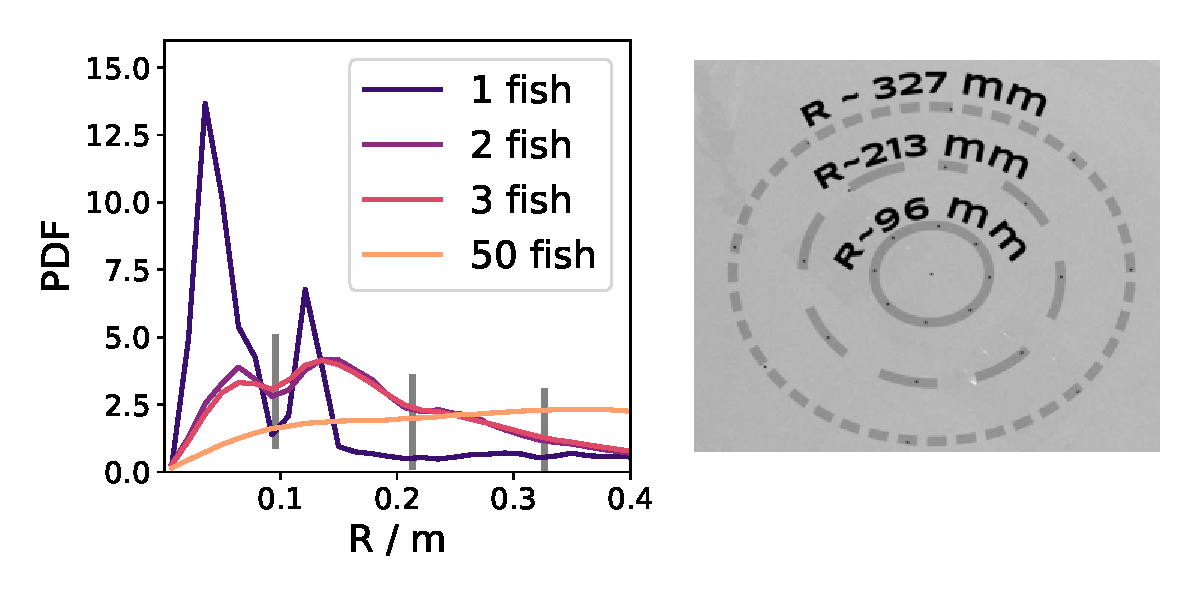
\includegraphics[width=\linewidth]{density-hole}
  \caption[The effect of drilled holes on the tank on the spatial distribution of the fish.]{
  	Left: the distribution of the planar radius ($R$), where the location of the drilled holes were marked with vertical lines.
  	Right: a photo of the bottom of the fish tank, highlighting the location and planar radius of the holes.
  }
  \label{fig:density-holes}
\end{SCfigure}

\vfill
\pagebreak

%\section{Conclusion}
%
%This chapter provides an introduction for the calculation of fish location in 3D from a multiple view system. The methods section gives an overview of the hardware design as well as the software design. Especially, the mathematical basis as well as the algorithm for the 3D locating problem is given explicitly, where the reader should be able to understand and implement a similar software for the same task. The performance and accuracy of my implementation was reported, suggesting the code is capable of processing a relatively large ($n \sim 50$) group of fish.
%
%Using the developed hardware and software, I present the spatial distribution of 1/2/3 and 50 fish. These distribution were inhomogeneous, being similar to the results observed in the quasi-2D experiment reported in chapter~\ref{chapter:fish_2d}. Surprisingly, the fish responded strongly to the small holes drilled in the tank, leading to characteristic peak split in the marginal distribution of the planar radius of the fish. For 50 fish, the interaction between the fish and the holes were not observable, indicating the behaviour of 50 were dominated by the fish-fish interaction. The interaction between the fish and the environment, otherwise, contributes significantly to the 1/2/3 fish behaviour.

\begin{adjustwidth}{0cm}{-5cm}
\begin{tcolorbox}[
fonttitle=\sffamily\Large,
right=0.1\linewidth,
top=5mm,
bottom=5mm,
title=Summary of Chapter~4,
]

\begin{itemize}
	\item Locating fish in 3D requires synchronised images from different cameras. We Presented the experimental setup for this task.
	\item We introduced the idea to calculate the 3D location of one fish from its corresponding 2D features from different cameras.
	\item We presented a brute-force algorithm to locate multiple fish in 3D, highlighting the importance of the reprojection error. We also introduced the optimisation of the result with the help of linear programming. The accuracy and complexity of the multiple-fish locating algorithm is assessed.
	\item We reported the analysis on the coordinates of zebrafish in a 3D environment, featuring different fish numbers.
	\begin{description}
		\item[One Fish] \hfill \\
		The fish tend to swim near the bottom of the tank. The height distribution exhibit an exponential decay, featuring the depth preference of the fish, which can be characterised by a length scale $\xi_g$.
		\item[Two Fish] \hfill \\
		The fish tend to swim near the bottom of the tank, with slightly increased $\xi_g$ value, suggesting a reduced depth preference. The depth preference dominated the radial distribution function.
		\item[Three Fish] \hfill \\
		The behaviour of three adult zebrafish is very similar to that from two fish.
		\item[Fifty Fish] \hfill \\
		The spatial distribution of 50 fish is more uniform, compared to the 1/2/3 fish results. As a result, the RDF of 50 zebrafish shows significantly reduced cohesiveness.
	\end{description}
	\item Surprisingly, the fish responded strongly to the small holes drilled on the surface of the tank, leading to the peak split in the distribution of the planar radius, for the 1/2/3 fish behaviour. For 50 fish, the interaction between the fish and the holes was not observable, indicating the behaviour of 50 zebrafish were dominated by the fish-fish interaction, instead of the interaction between the fish and the environment.
\end{itemize}
\end{tcolorbox}

\end{adjustwidth}


\end{document}
